\documentclass{article}
\usepackage{amsmath,amsthm,amssymb,amsfonts}
\usepackage{setspace,enumitem}
\usepackage{graphicx}
\usepackage{hyperref}
\usepackage{natbib}
\usepackage{afterpage}
\usepackage{xcolor}
\usepackage{etoolbox}
\usepackage{booktabs}
\usepackage{pdfpages}
\usepackage{multicol}
\usepackage{geometry}
\usepackage{accents}
\usepackage{bbm}
\usepackage{placeins}
\usepackage{verbatim}
\usepackage{csvsimple}
\hypersetup{
	colorlinks,
	linkcolor={blue!90!black},
	citecolor={red!90!black},
	urlcolor={blue!90!black}
}

\newtheorem{theorem}{Theorem}
\newtheorem{assumption}{Assumption}
\newtheorem{definition}{Definition}
\newtheorem{lemma}{Lemma}
\setlength{\parindent}{0cm}
\geometry{margin = 1in}

\newcommand{\R}{\mathbb{R}}
\newcommand{\ubar}[1]{\underaccent{\bar}{#1}}
\newcommand{\Int}{\text{Int}}
\newcommand{\xbf}{\mathbf{x}}
\newcommand{\Abf}{\mathbf{A}}
\newcommand{\Bbf}{\mathbf{B}}
\newcommand{\Gbf}{\mathbf{G}}
\newcommand{\bbf}{\mathbf{b}}
\newcommand{\one}{\mathbbm{1}}

\newtoggle{extended}
\settoggle{extended}{false}

\title{ECON 717B: PS 1}
\author{Alex von Hafften}

\begin{document}

\maketitle

\section{Part 1: Analytic Exercises}

\begin{enumerate}

\item Returns to schoolings

\begin{enumerate}

\item ATE

Marginal treatment effect is

$$
MTE(A) = Y_1(A) - Y_0(A) = 1 + 0.5A - A = 1 - 0.5A
$$

Average treatment effect is

$$
E[MTE(A)] = E[1 - 0.5A] = 1 - 0.5E[A] = 1 - 0.5*0.5 = 0.75
$$

\item Fraction of treated population

$$
Pr\{D = 1\} = Pr\{-0.5 + A > 0 \} = Pr\{A > 0.5 \} = 0.5
$$

\item Maximum and minimum treatment effect

$$
\max_{A \in [0,1]} MTE(A) = \max_{A \in [0,1]} [1 - 0.5A] = 1
$$

at $A = 0$.

$$
\min_{A \in [0,1]} MTE(A) = \min_{A \in [0,1]} [1 - 0.5A] = 0.5
$$

at $A = 1$.


\item $A \sim N(0, 1)$

$$
\sup_{A \in (-\infty,\infty)} MTE(A) = \sup_{A \in (-\infty,\infty)} [1 - 0.5A] = \infty
$$

as $A \to -\infty$.

$$
\inf_{A \in (-\infty,\infty)} MTE(A) = \inf_{A \in (-\infty,\infty)} [1 - 0.5A] = -\infty
$$

as $A \to \infty$.

\item ATET and ATEU

$$
ATET = E[MTE(A) | D = 1] = E[1- 0.5A | A > 0.5] = 1- 0.5 E[A | A > 0.5] = 1 - 0.5*0.75 = 0.625
$$

$$
ATEU = E[MTE(A) | D = 0] = E[1- 0.5A | A < 0.5] = 1- 0.5 E[A | A < 0.5] = 1 - 0.5*0.25 = 0.875
$$

\item Why is ATEU $>$ ATET?

ATEU $>$ ATET because the marginal treatment effect is decreasing in $A$, but selection into treatment is increasing in $A$.

\item OLS estimand

$$
\beta(OLS) = E[Y|D=1] - E[Y|D=0] = E[1 + 0.5A |A > 0.5] - E[A|A < 0.5] = 1 + 0.5 *0.75 - 0.25 = 1.125
$$

\item Why is OLS biased upward for ATE?

Because conditional independence fails due to selection effects.  If treatment was random, then OLS would be unbiased.

\end{enumerate}

\item Monotonicity

\begin{enumerate}

\item Prove monotonicity holds.

For each observation $i$, define $V_{0,i} \equiv \delta_0 + U_{V,i}$ as the outcome without treatment and $V_{1,i} \equiv \delta_0 + \delta_1 + U_{V,i}$ as the outcome with treatment.

Case 1: $\delta_1 > 0 \implies \delta_0 + \delta_1 + U_{V,i} > \delta_0 + U_{V,i} \implies V_{1,i} > V_{0,i}$ for all $i$. Monotonicity holds.

Case 2: $\delta_1 < 0 \implies \delta_0 + \delta_1 + U_{V,i} < \delta_0 + U_{V,i} \implies V_{1,i} < V_{0,i}$ for all $i$. Monotonicity holds.

Case 3: $\delta_1 = 0 \implies\delta_0 + \delta_1 + U_{V,i} = \delta_0 + U_{V,i} \implies V_{1,i} = V_{0,i}$ for all $i$. Monotonicity holds.

\item Define $V$ such that monotonicity fails.

Consider heterogenous $\delta_{1,i} \in [-A, A]$:

$$
V_i = \delta_0 + \delta_{1,i} Z_i + U_{V, i}
$$

Since $\delta_{1,i}$ can be positive or negative, defier will not choose the treatment even if they are exposed to the instrument.

\end{enumerate}

\item Potential outcomes with uniform instrument

\begin{enumerate}

\item Show range of always takers, compliers, defiers, and never takers.

Monotonicity holds, so there are no defiers. Always takers have $V > 0$ for both $Z = 0$ and $Z = 1$, so $U_V \in [0, 2]$. Compliers $V > 0$ for $Z = 1$, but $V < 0$ for $Z = 0$, so $U_V \in [-1, 0)$. Never takers have $V < 0$ for both $Z = 0$ and $Z =1$, so $U_V \in [-2, -1)$. The figure below summarizes these ranges:

\begin{center}
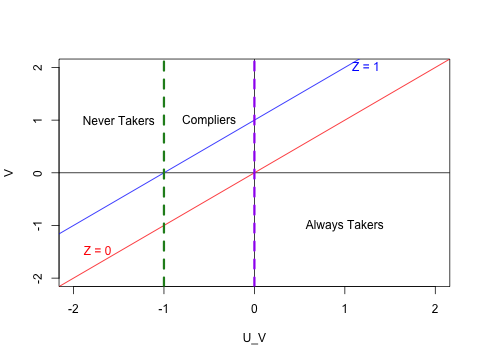
\includegraphics[scale = 0.8]{p1_q3_a}
\end{center}

\item Compute fraction of population in each group.

Using the uniform distribution, defiers are 0 percent, always takers are 50 percent, compliers are 25 percent, and never takers are 25 percent.

\end{enumerate}

\item Two types

\begin{enumerate}

\item Compute ATE

...

\item Compute $Pr(D=1 | Z = 1)$ and $Pr(D=1 | Z = 0)$

...

\item Compute LATE

...

\end{enumerate}

\end{enumerate}

\section{Monte Carlo Exercises}

\subsection{Question 1}

...

\subsection{Question 2}

...

\end{document}